%Note di Ingegneria del Software
%Sommario: Classi Astratte, Interfacce, Diagrammi di Package, Diagrammi di Attività

\cornell{Classe Astratta}{Non istanziabile.\\
Ha alcuni metodi astratti (Senza Implementazione), mentre altre operazioni possono avere implementazione.\\
Le classi ed i metodi astratti vanno scritti in corsivo.\\
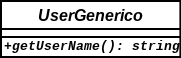
\includegraphics[scale=0.5]{images/34.png}\\
Dato che a mano è difficile distinguere tra corsivo e normale, è possibile fare uso delle proprietà aggiuntive per distinguere le classi astratte da quelle concrete:\\
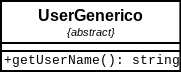
\includegraphics[scale=0.5]{images/35.png}\\
(Nota: Le proprietà aggiuntive vanno messe \textbf{tra parentesi graffe} e non doppie parentesi angolari)\\
Quando si va ad implementare un metodo in una classe concreta, questo \textbf{va scritto} (al contrario dei casi di ereditarietà)
}

\cornell{Interfaccia}{Classe priva di implementazione.\\
Una classe realizza un'interfaccia se ne implementa le operazioni. Negli schemi UML 2.x le interfacce sono rappresentate con un "lecca lecca":\\
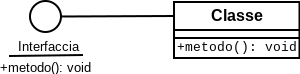
\includegraphics[scale=0.5]{images/36.png}\\
Mentre in UML 1.x si fa uso della parola chiave nativa di UML \lstinline{<<interface>>}\\
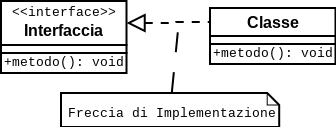
\includegraphics[scale=0.5]{images/37.png}\\
Essendo una parola chiave nativa (e non una proprietà aggiuntiva) interface va scritto \textbf{tra parentesi angolari doppie}.\\
I metodi delle interfacce sono sempre pubblici.}

\cornell{Estensione Tra Interfacce}{È possibile che alcune interfacce estendano da altre interfacce:\\
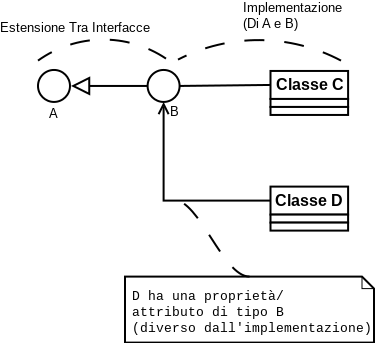
\includegraphics[scale=0.5]{images/38.png}}

\cornell[Attenzione]{Estensione? Implementazione?}{Per sapere se qualcosa implementa o estende un'interfaccia, è sufficiente fare riferimento ai significati di Java di "Extends" ed "Implements".\\
Un'interfaccia può estendere un'altra interfaccia (ereditarietà) oppure una classe può implementare un'interfaccia (realizzazione)}

\cornell{Creazione di Istanze}{Se ho uno schema in cui si va a creare un'istanza di una classe che implementa un'interfaccia, posso usare una forma contratta per rendere meno caotico lo schema. Quindi questa forma:\\
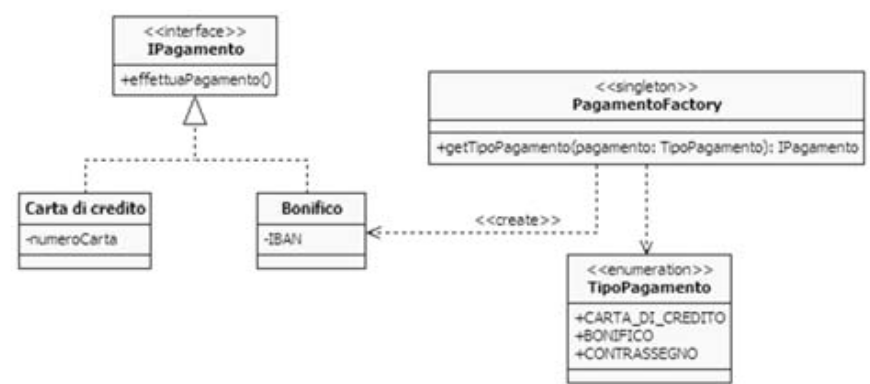
\includegraphics[scale=1.0]{images/39.png}\\
E questa:\\
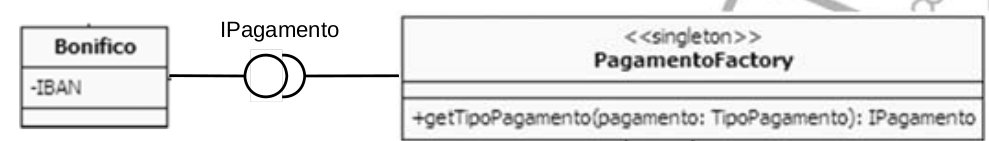
\includegraphics[scale=0.3]{images/40.png}\\
Vogliono dire esattamente la stessa cosa.}

\cornell{Varie}{In UML, le operazioni e gli attributi statici vanno sottolineati nel diagramma:\\
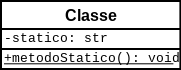
\includegraphics[scale=0.5]{images/41.png}\\
Si possono aggiungere altri box all'interno delle classi, oltre agli attributi ed alle operazioni si possono avere box dedicati alle Eccezioni Lanciate (Exceptions) ed ai contratti delle classi (Responsibilities)\\
Inoltre si possono aggiungere parole chiave e proprietà aggiuntive, un esempio è:\\
\lstinline{<<enum>>} che definisce classi enumeratore (tenere conto che ogni attributo di classi enum è pubblico.)\\
Inoltre vi è una parte dedicata ai generics/template/classi con tipo parametrico, che possono essere rappresentate in questo modo:\\
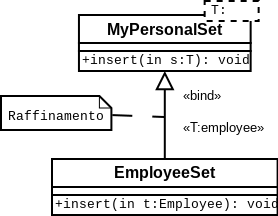
\includegraphics[scale=0.5]{images/42.png}\\
Inoltre è utile ricordare le classi attive, che eseguono e controllano un proprio thread, la rappresentazione in UML 2.x è:\\
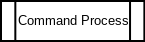
\includegraphics[scale=0.5]{images/43.png}\\
In UML 1.x si ingrossava il bordo del box "classe", ma questo rendeva solo lo schema più confuso.}
\cornell{Consigli}{Si consiglia di evitare diagrammi troppo ricchi, in quanto sono poco utili, confondono le idee e troppi dettagli portano a troppi concetti da modificare nel caso si andassero ad aggiungere feature o modifiche di codice.\\
È opportuno iniziare esponendo concetti semplici.}
\cornell{Diagrammi dei Package}{Sono Un modo di raggruppare elementi UML (solitamente classi) in unità di livello più alto.\\
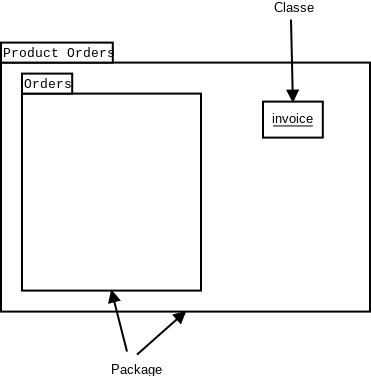
\includegraphics[scale=0.3]{images/44.png}\\
Dei package possono essere contenuti in altri package, con l'unica condizione che \textbf{non vi siano condivisioni tra package} (una classe può stare in un solo package), ogni package determina un namespace, quindi si possono avere situazioni con ugual nome, ma in package diversi; tipo:\\
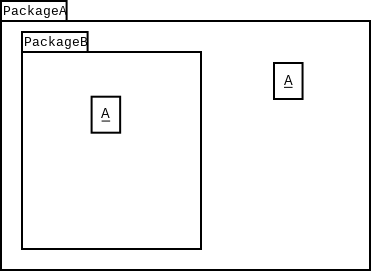
\includegraphics[scale=0.3]{images/45.png}\\
Inoltre È possibile far uso dei nomi completamente qualificati per semplificare lo schema, soprattutto nel caso non si debba far uso di tutto il pacchetto, o addirittura sia necessaria solo una classe.\\
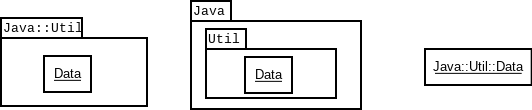
\includegraphics[scale=0.5]{images/46.png}\\
Un'altra possibile notazione per I package in UML 2.x è:\\
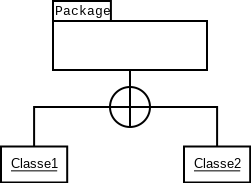
\includegraphics[scale=0.5]{images/47.png}}

\cornell{Visibilità nei package}{Solo Pubblica o privata:\\
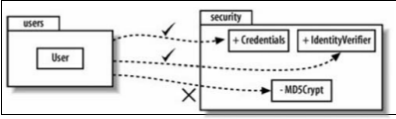
\includegraphics[scale=0.5]{images/48.png}}

\cornell{Interfaccia di un package}{Insieme dei metodi pubblici delle classi con visibilità pubblica che stanno all'interno di un certo package.}

\cornell{Principi di progettazione}{Quando si tratta di progettare i pacchetti, solitamente si fa riferimento ad uno di due principi: \begin{description}
\item [Common Reuse Principle] Si mettono nello stesso package le classi che solitamente sono riusate insieme
\item [Common Closure Principle] Si mettono nello stesso package le classi che hanno lo stesso obiettivo
\end{description}\\
L'uso di un principio o l'altro è questione di preferenze, ma solitamente si preferisce quello che permette di disegnare package più piccoli.\\
Il principio \textbf{common reuse} (solitamente) rende più semplice individuare ed attuare modifiche tra classi che presentano delle interdipendenze}

\cornell{Il diagramma}{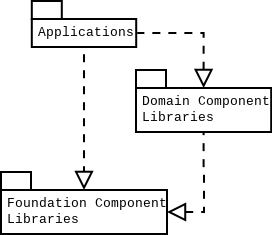
\includegraphics[scale=0.5]{images/49.png}\\
Il diagramma documenta le dipendenze fra le classi ed aiuta ad identificare, evitare e "rompere" eventuali \textbf{dipendenze circolari}.\\
I diagrammi di package dovrebbero presentarsi come grafi aciclici.\\
Inoltre è importante ricordare che le relazioni di dipendenza \textbf{non sono transitive}: se ho una classe C che dipende da B che a sua volta dipende da A, non è detto che se modifico A debba modificare anche C.}

\cornell{Rompere le dipendenze circolari}{È possibile rompere le dipendenze circolare in 2 modi: \begin{description}
\item [Fattorizzazione] Creare un terzo pacchetto, da cui dipendono i primi due, che permetta di esternalizzare ciò che rendeva i due pacchetti interdipendenti
\item [Riduzione] Due pacchetti interdipendenti potrebbero essere prodotto di una fattorizzazione troppo forzata, ed i contenuti potrebbero in realtà stare meglio se sono nello stesso pacchetto
\end{description}}

\cornell{Package di Interfaccia}{Contengono interfacce e classi astratte:\\
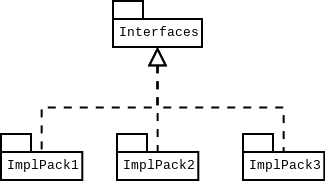
\includegraphics[scale=0.5]{images/50.png}}
\cornell{Diagrammi di Attività}{Sono un raffinamento dei vecchi "diagrammi di flusso:"\\
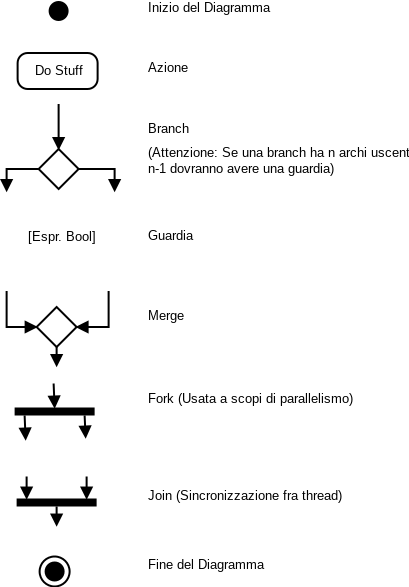
\includegraphics[scale=0.5]{images/51.png}}

\cornell{Consigli}{Evitare diagrammi troppo grandi, i diagrammi di attività vanno a modellare \textbf{un singolo processo}}

\cornell{Esempio: Ordine su Amazon}{ 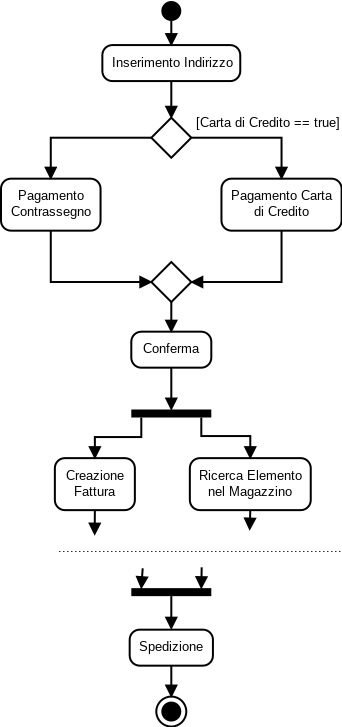
\includegraphics[scale=0.5]{images/52.png} }

\cornell{Nodo Di Fine Flusso}{Usato per interrompere un thread senza necessità di usare una join, in questo caso allora la Join dovrà necessariamente avere una guardia\\
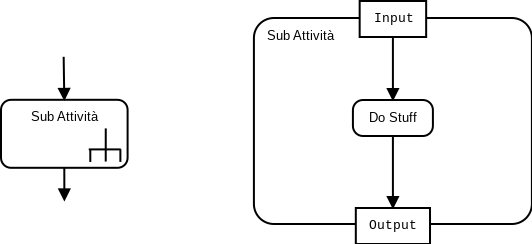
\includegraphics[scale=0.5]{images/53.png}}

\cornell{SubAttività}{Permettono di dettagliare attività complesse, l'input ed output delle sottoattività sono rappresentati da dei rettangoli.\\
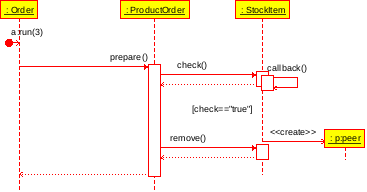
\includegraphics[scale=0.5]{images/54.png}}
